\documentclass{article}
\usepackage{graphicx}
\begin{document}

\author{S. Dorsher}
\title{Phrase Quest}

\maketitle

Wouldn't it be fun if you could create a phrase and generate a
latitude and longitude? You could meet a friend at ``You could meet a
friend'', ``Hello Ma'am???'', ``Does anyone want to play Seven
Wonders?'', ``Ufda, well that about does it'', or ``l33t h4ck3rs''. It is my belief that all of these sentiments contain some geographic information, in addition to their mood information. Probably that information is both regional and relates to small towns versus large towns. To assess it, I propose to make use of the distribution of characters in airport names. 

I have obtained airplane data from the OpenFlights Airport Database on
April 21, 2018. The important fields, for my purposes, are Airport
Name, specified in Unicode-8, possibly City and Country for
exploratory purposes, and Latitude and Longitude. It is fairly obvious
that in many, but not all, cases languages correlate with countries or
groups of countries; thus, certain character sets within Unicode-8
also correlate with those countries. However, it seems to be possible
to convert vowels, consonants, symbols, and spaces in a fairly
universal manner at least for the Romance and Germanic languages using
case insensitivity in python.

I ultimately propose to classify languages into regions using
clustering based on airport names, train terminals, and bus stops in
the basic list airports\_extended.dat, limiting the data to the United
States. I will use python and tensorflow to do this. The training set
will be airports.dat, which uses world data limited only to airports.

Some preliminary data analysis is included below, based on airport
data from around the world in the smaller file
airports.dat. Figure~\ref{fig1} was created by counting the vowels and
consonants in each airport name, producing the ratio, and sorting in
descending order. The spike at the left is due to low numbers of
consonants, approaching a minimum. The sudden drop at the right is due
to low numbers of vowels, approaching a minimum. These are properties
of the ratio and the discreteness of vowel and consonant
quantities. Figure~\ref{fig2} demonstrates that the behavior of the
curve is qualitatively similar for six countries sampled,including
countries using at least one foreign language, such as France,
Germany, or Mexico. The control, Canada, was in fact intermediate
between the United States and France. Figure~\ref{fig3} demonstrates
that this behavior is third order polynomial, and thus a third order
feature would be required. 

Further exploratory data analysis will be necessary to determine the
scaling of the additional features dependent upon symbol to consonant
ratio and space to consonant ratio. I will also need to make
assumptions about the scaling at smaller physical scales within a
country to extend the data from airports.dat to airports\_extended.dat.

After I have mapped the world by language clusters, it will be
possible to input a sentence or phrase function and output a longitude
and latitude. You could tell a partner to meet them at ``I love you''
or at the date of your engagement.  It could be like Pokemon Go or
GeoCaching. Families and friends could play, and make a car trip or plane ride of it.

\begin{figure}
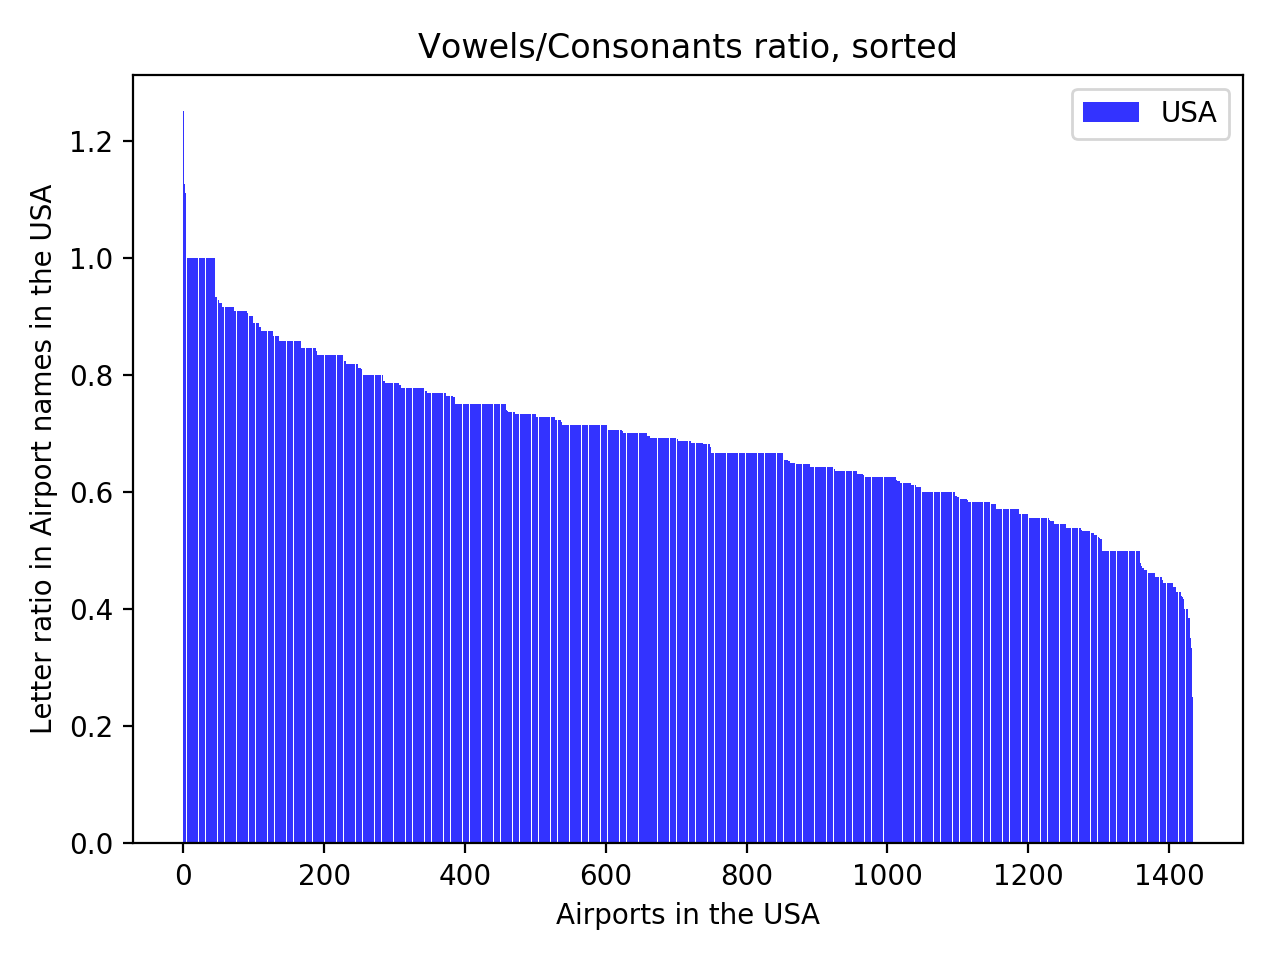
\includegraphics[width=4.0in]{USAhistogramVtoChist.eps}
\caption{Sorted histogram of the Vowel to Consonant Ratio for airports within the USA.}
\label{fig1}
\end{figure}

\begin{figure}
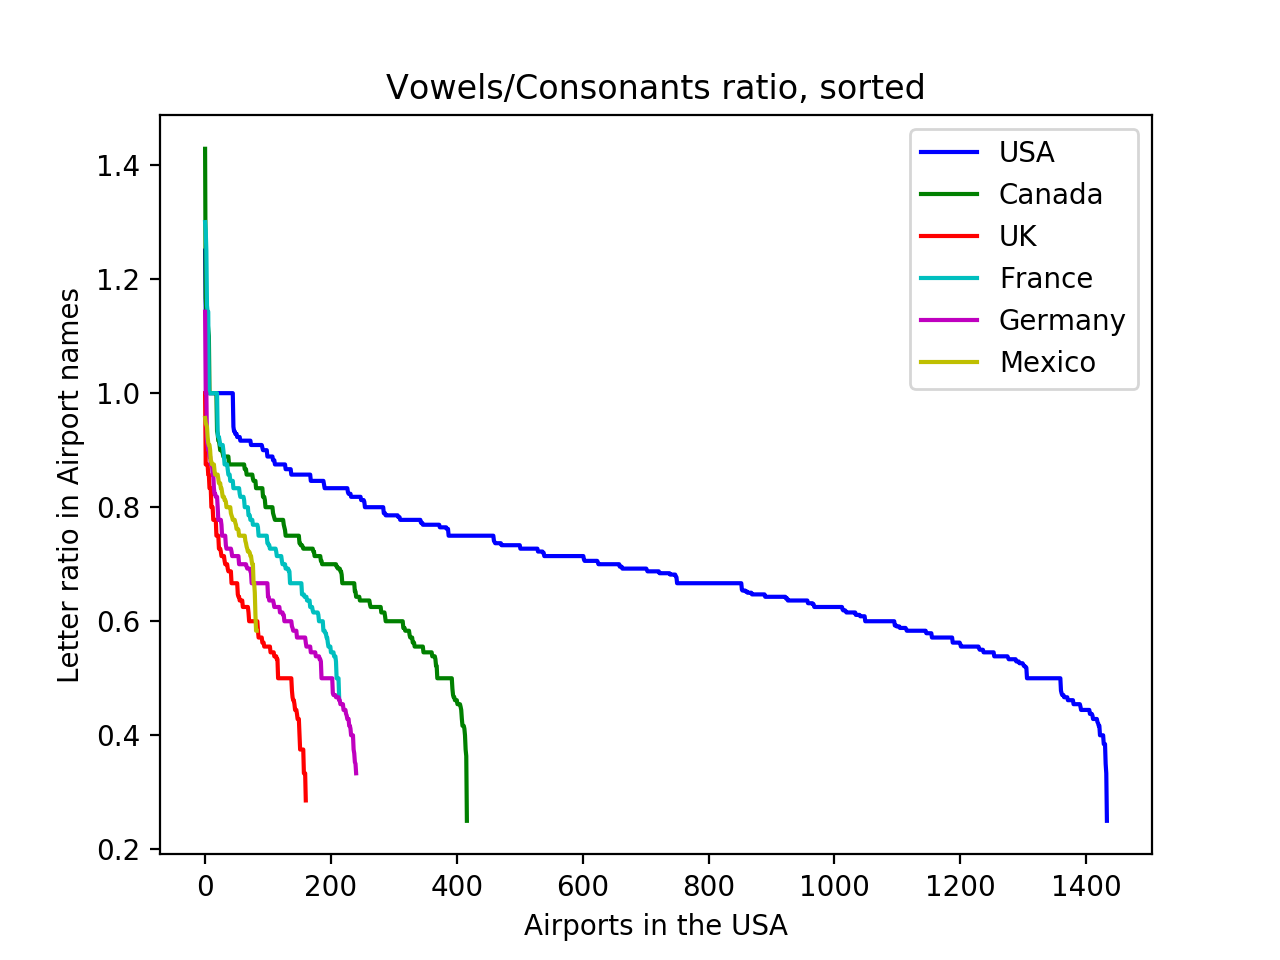
\includegraphics[width=4.0in]{VtC6countries.eps}
\caption{Sorted histograms of the Vowel to Consonant Ratio for airports in 6 different countries using 4 different languages, with a case insensitive vowel count. Different countries have dramatically different PDFs.}
\label{fig2}
\end{figure}

\begin{figure}
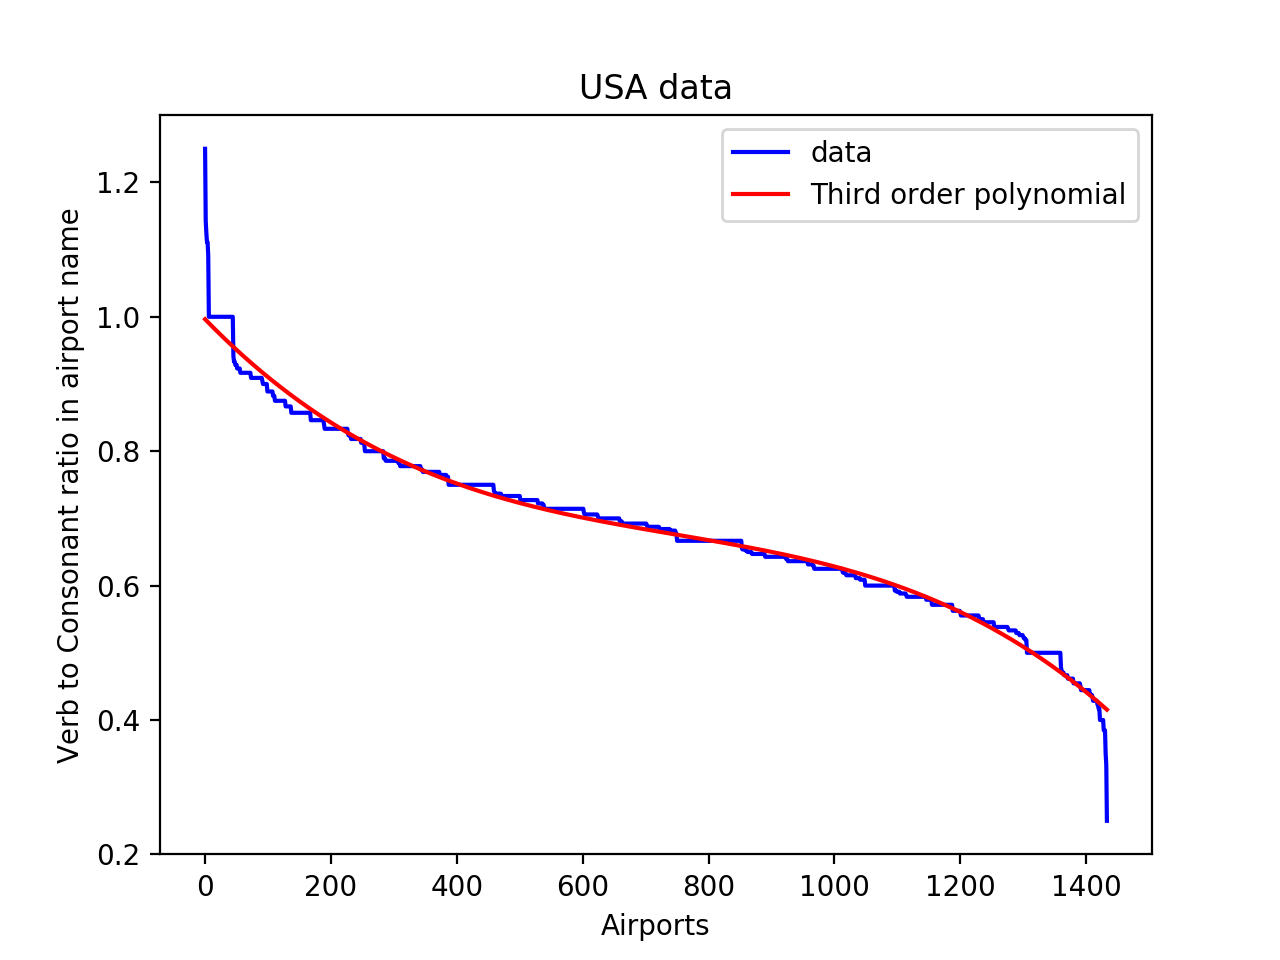
\includegraphics[width=4.0in]{Fitto3rdOrder.eps}
\caption{The United States distribution is well fit by a third order polynomial. This implies that a model will require third order contributions in this feature.}
\label{fig3}
\end{figure}


\end{document}
